\section{Server Design}
\label{ServerDesign}

The GIM server is primarily responsible for synchronising the communication between the connected clients and keeping a persistent record of user information. In particular the server is responsible for:

\begin{itemize}
    \item{Authenticating users}
    \item{Routing chat messages for one client to one or more other clients}
    \item{Sending requests from one client to another client (such as friend requests or chat invites)}
    \item{Notifying subscribed users of changes to another user's information}
    \item{Storing user information such as nicknames, passwords, display pictures, friend lists, etc.}
\end{itemize}

This section discusses how the design of the server copes with these requirements and the the reasoning behind these decisions.

\subsection{Server Structure}

From the very beginning the server was designed to be secure, scalable, and simple. Users must trust it to keep their information safe and route messages correctly, and it must be able to cope with any number of connected clients.

In order to manage this, the server generates a new worker for every connected client, as shown in figure \ref{WorkersDia}. This new worker acts as the single point of contact for its respective client. This greatly simplifies the design of the server as we can treat each connection individually and allows the server to easily scale to a large number of clients.

\begin{figure}
    \begin{center}
        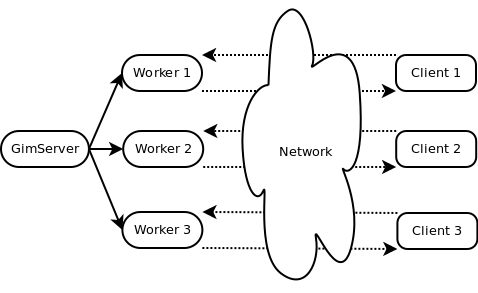
\includegraphics[scale=0.6]{Design/diagrams/server_workers.png}
        \caption{The GIM Server with 3 connected clients, each with their own worker.}
        \label{WorkersDia}
    \end{center}
\end{figure}

Each worker has two buffers, one which stores commands read from the network (the command buffer), and one which stores commands to be written to the network (the response buffer). The worker continually reads commands from the command buffer, processes them, and puts the responses into the response buffer. At the same time the worker is also performing network reads and writes to fill and empty the respective buffers. This is show in figure \ref{WorkerDatailedDia}.

The buffers allow the worker to run using several threads which increases the performance on multi-core systems as the server is able to read from the network, process commands, and write to the network in a truly concurrent fashion. This means that at any one time a worker could be handling up to three different commands, each at a different stage of execution, and still have several commands stored in the buffers waiting to be used.

\begin{figure}
    \begin{center}
        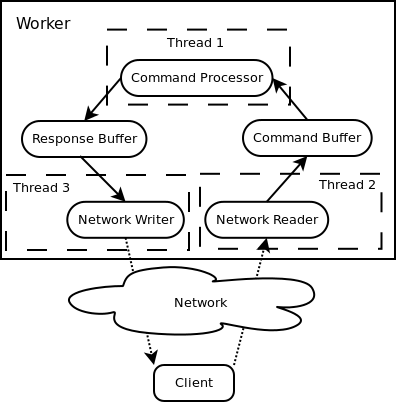
\includegraphics[scale=0.6]{Design/diagrams/worker_detail.png}
        \caption{The internal components of a single worker.}
        \label{WorkerDatailedDia}
    \end{center}
\end{figure}

\subsection{User Accounts}
A user is a registered account on the server with a unique identifier (an email address), password, nickname, personal message, display picture, status, and friend list. 

\begin{itemize}
\item{{\bf Identification}\\
The user's identifier and password are used to authenticate the user at login. These cannot be changed one the account has been created.} 

\item{{\bf Nickname}\\
A user's nickname is a short and familiar name for that user. A nickname does not need to be unique and is not intended to be used as an identifier by the system. By default a user's nickname is their email address.}

\item{{\bf Personal Message}\\
The personal message is a medium length message (usually only a sentence or two) which the user can use to share news or any information about themselves.}

\item{{\bf Status}\\
A user can have one of several statuses: Online, Away, Busy and Appear Offline. The first three statuses are used simply as an indication of the user's likelihood to respond to a message. The Appear Offline status allows the user to appear to other users as though they were not signed in but still receive updates and messages from other users.}

\item{{\bf State}\\
A user can have one of only two states, Online or Offline. States should not be confused with a user's status. A users status is simply an abstract representation, picked by the user, while a users state is an internal representation of the actual online state of the user. A user is only considered to be Online if they are connected using a client, and that client has logged-in successfully, otherwise they are considered to be Offline.}

\item{{\bf Friend List}\\
Each user has their own Friend List, a list of users who have accepted a friend request from the owner of the Friend List. When a user accepts a friend request, the sender and receiver are added to each other's Friend List.}
\end{itemize}



\subsection{Client-to-Client Messaging}
\label{c2c}
No direct client-to-client communication is possible. However, workers and (in an ad-hoc fashion) clients are able to indirectly communicate with other clients (i.e. clients to which they are not connected) by passing commands to the other client's worker. This is the server's main method of inter-client communication and relies heavily on the use of the buffers to pass messages from one worker to the network writer or command processor of another worker.

As the protocol defines no client to client communication is possible before a user has logged in, and as user can only be logged in on one client at a time, only a user id is necessary to send a command to a user. As long as a record is kept of which worker belongs to each online user, then sending a message to a user is no more complicated than identifying the particular user.

\subsection{Rooms and Message Routing}
\label{message_routing}

Message routing in the server is fairly simple because of the use of rooms. A room is a collection of one or more users and each room has a unique identifier. In order to join a room a user must either create a new room (in which case they are automatically placed into the room) or they must be invited to the room by a user already in the room. A room can be one of two types: personal or group. A personal room is much more restrictive than a group room. A personal room must be provided with the identifier of one other user at time of creation and is limited to only 2 users. Once a personal room has been created you cannot invite any other users. A group room has no such restrictions. Any number of users may be invited to a group room at any time.

All chat messages in GIM are sent to Rooms rather than particular users. The server must maintain a list of the users in each room, and upon receipt of a message for that room, forward it to all of the users in the room (excluding the sender of the message). This is done using the method described in section \ref{c2c}. A \texttt{:MESSAGE:} command is generated and placed into the Response Buffer of the worker assigned to each of the recipients ready for the worker to send to the client.

\subsection{Subscriptions, Privacy and Notifications}
One of the server's most critical responsibilities is notifying users of changes to other users. This is done using the concept of subscriptions. A user (the subscriber) is considered to be subscribed to another user (the subscribee) if they meet at least one of two conditions:

\begin{enumerate}
\item{The subscriber has the subscribee in their friend list, or had them in their friend list at some point in the past}
\item{Both the subscriber and subscribee are in the same room}
\end{enumerate}

When a user changes any piece of their user information such as their status, nickname, or personal message, the server needs to notify other clients so that they can update their information. The server generates a list of subscribers for this user and removes offline and blocked users. It then issues an \texttt{:UPDATE:} command to each of the clients, notifying them of the user and the piece of information which has been updated. Note that the server does not send the updated information, it merely notifies the client of the update, allowing it to request the updated information for the server when and if it needs it.

Subscriptions are also used as a method of access control. A user is only able to request information about another user if they are subscribed to that user. This limitation means that a user is effectively granting another user access to read their information by adding them to their friend list. However, the converse is not true. Removing a user from your friend list does not remove their access to your information as they may still have you in their friend list. In order to combat this, you are able to block a user which removes this access to your information and status updates. This enhances privacy and gives the user control of who is able to access their data.

\subsection{Synchronisation}
The server has a large section of backing data which stores all of the users, rooms, workers and any other operational data required by the server. Due to the highly concurrent nature of the server it is very important to ensure that the data is properly synchronised. This is to prevent race conditions where two writes occur on an object at the same time giving an unpredictable output, as show in \ref{RaceConditionDia}.

\begin{figure}
    \begin{center}
        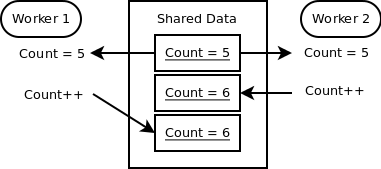
\includegraphics[scale=0.6]{Design/diagrams/server_race_condition.png}
        \caption{Unsynchronised workers updating the same object at the same time, resulting in a race condition and giving the unexpected value of 6 rather than 7.}
        \label{RaceConditionDia}
    \end{center}
\end{figure}

To stop this the server must lock (claim ownership of) the data before it is updated. This is a very tricky thing to do as as the lock must be long enough to ensure that no updates occur between reading the original data and writing the updated data, while also keeping the lock as short as possible to avoid long periods of blocking and keep performance high.

The server must also make sure only to lock when needed, and not obtain a lock for objects it does not require. This simplest solution would be to lock the entire data object, and only allow reads and writes through a proxy. However this would be extremely costly in terms of performance as writes to individual objects inside the data object would block writes to other objects, meaning that at any one time only a single write could occur. Instead the data object must be clever and only lock the objects which are to be written to, allowing for simultaneous writes to separate objects while still stopping race conditions from occurring.

\begin{figure}
    \begin{center}
        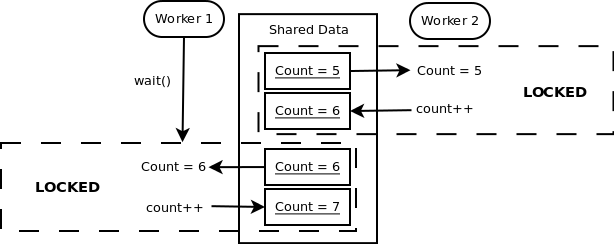
\includegraphics[scale=0.6]{Design/diagrams/server_locking.png}
        \caption{Synchronised workers using locking to read and write the updated value, giving the expected value of 7.}
        \label{lockingDia}
    \end{center}
\end{figure}

\subsection{The Controller and Timeout Manager}
Even though the server should be capable of functioning autonomously, some of the features defined by the protocol require interaction with the server that deviates from the client-server model. For example, the \texttt{:BROADCAST:} command allows the server to send a message to all of the clients it is connected to. The controller allows authorised users to interact through a command line interface with the server. These authorised users are allowed by the operating system to connect to the session that is running the server. They are then able to execute several commands defined by the controller to broadcast messages and control the server. These commands are independent from protocol commands.

For example, the \texttt{:QUIT:} command tells the server to shut down and create a persistence file to store user data, and the following would send a \texttt{:BROADCAST:} command to all of the connected clients:

\texttt{BROADCAST We're shutting the server down in 15 minutes.}

The server needs to periodically check for clients which have not sent a command in the last 15 seconds (as defined in the protocol) and disconnect them. This means that the server must compare the time the last command was received by every worker with the current time. If the difference exceeds 15 seconds, they are disconnected.

Due to the nature of the Controller and Timeout Manager, they both must run on separate threads from the rest of the server or risk blocking a more important function, such as accepting incoming connections and creating workers for them.

\begin{landscape}
    \begin{figure}
        \begin{center}
            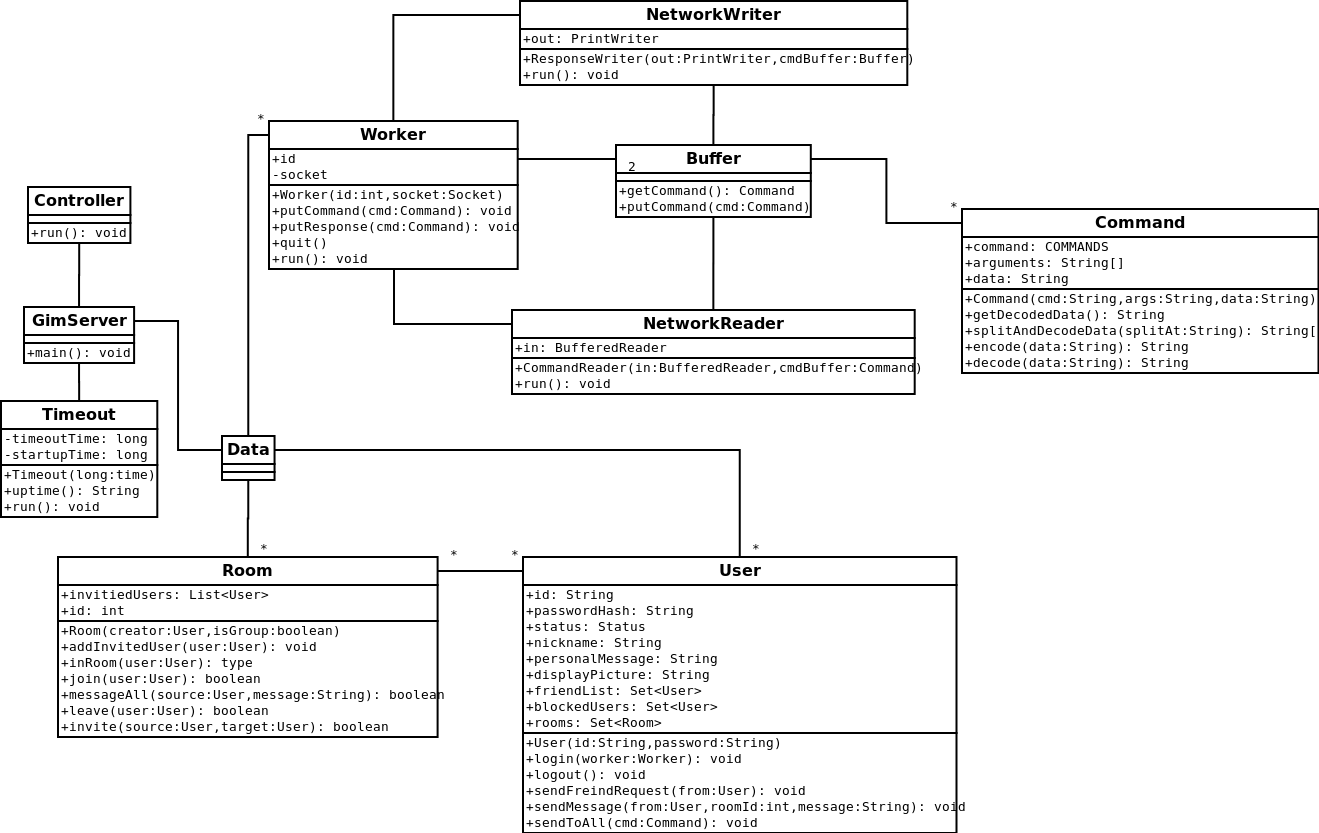
\includegraphics[scale=0.5]{Design/diagrams/server_uml.png}
            \caption{UML showing the structure of the GIM Server.}
            \label{umlDia}
        \end{center}
    \end{figure}
\end{landscape}
